\documentclass{article}
\usepackage{tikz}
\usepackage{pgf}
\usetikzlibrary{arrows,shapes,positioning,shadows,trees}

\tikzset{
  basic/.style  = {draw, text width=2cm, drop shadow, font=\sffamily, rectangle},
  level 1/.style = {basic, rounded corners=6pt, thin,align=center, fill=green!60,
                   text width=8em}
}

\begin{document}

\noindent
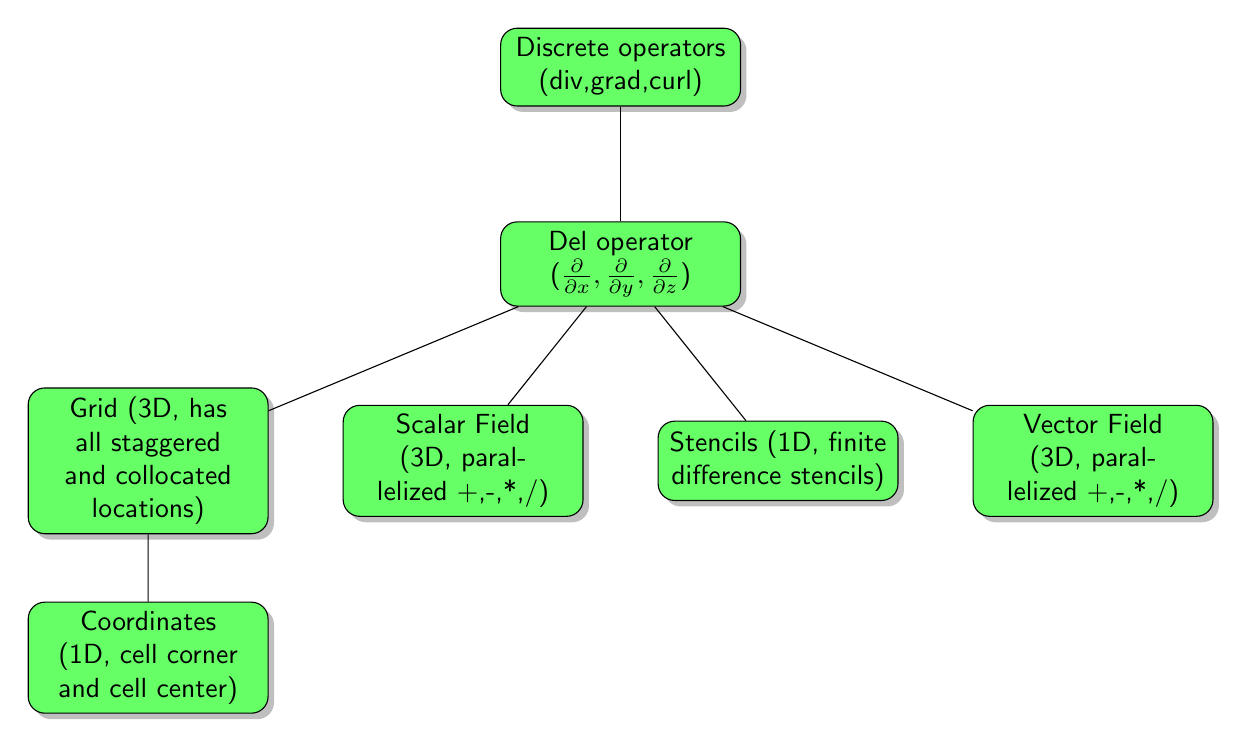
\begin{tikzpicture}[level distance=25mm,level/.style={sibling distance=40mm}]
\node[level 1] {Discrete operators (div,grad,curl)}
	child {
		node[level 1] (c1) {Del operator 
		($\frac{\partial }{\partial x},\frac{\partial }{\partial y},\frac{\partial }{\partial z}$)}
		child {
			node[level 1] (c2) {Grid (3D, has all staggered and collocated locations)
		}
		child {
			node[level 1] (c3) {Coordinates (1D, cell corner and cell center)}}
		}
		child {
			node[level 1] (c4) {Scalar Field (3D, parallelized +,-,*,/)}
		}
		child {
			node[level 1] (c5) {Stencils (1D, finite difference stencils)}
		}
		child {
			node[level 1] (c6) {Vector Field (3D, parallelized +,-,*,/)}
		}
	};
\end{tikzpicture}

\noindent
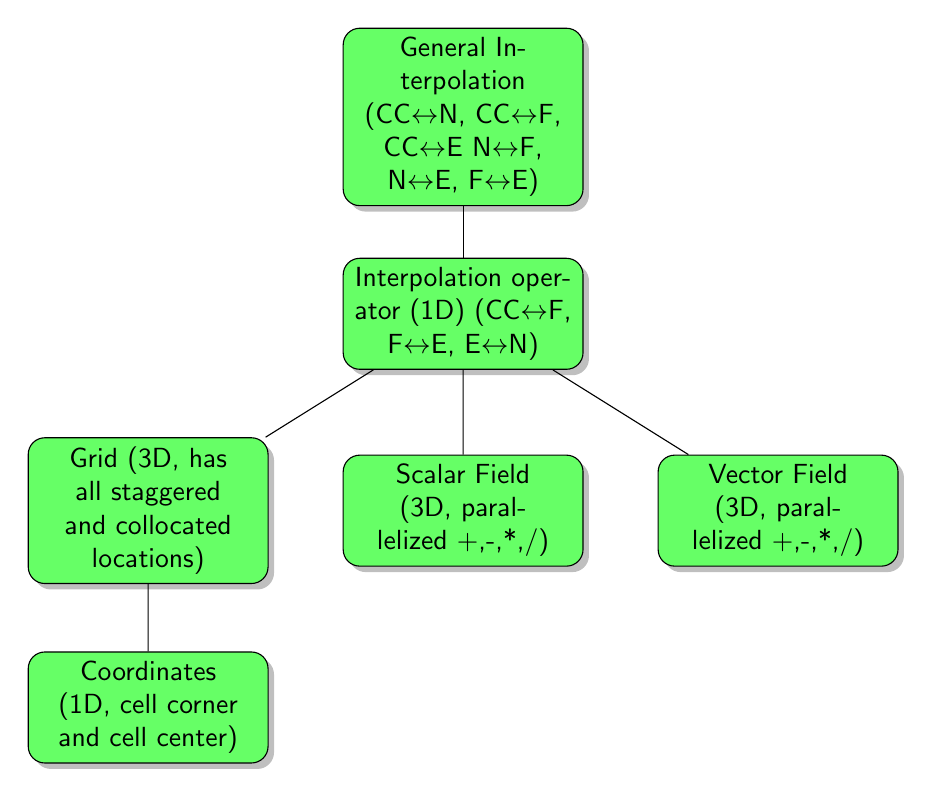
\begin{tikzpicture}[level distance=25mm,level/.style={sibling distance=40mm}]
\node[level 1] {General Interpolation
	(CC$\leftrightarrow$N, 
	CC$\leftrightarrow$F, 
	CC$\leftrightarrow$E
	N$\leftrightarrow$F, 
	N$\leftrightarrow$E, 
	F$\leftrightarrow$E)
	}
  child {node[level 1] (c1) {Interpolation operator (1D)
	(CC$\leftrightarrow$F, 
	F$\leftrightarrow$E, 
	E$\leftrightarrow$N)
  }
  child {node[level 1] (c2) {Grid (3D, has all staggered and collocated locations)}
  child {node[level 1] (c3) {Coordinates (1D, cell corner and cell center)}}}
  child {node[level 1] (c4) {Scalar Field (3D, parallelized +,-,*,/)}}
  child {node[level 1] (c5) {Vector Field (3D, parallelized +,-,*,/)}}};
\end{tikzpicture}



\end{document}